\documentclass[a4paper,12pt,twoside,openright,titlepage]{book}

%Additional packages
\usepackage[ascii]{inputenc}
\usepackage[T1]{fontenc}
\usepackage[dutch,english]{babel}
\usepackage{syntonly}
\usepackage[official]{eurosym}
%\usepackage[graphicx]
\usepackage{graphicx}
\graphicspath{ {./images/} }
\usepackage{float}
\usepackage{hyperref}
\hypersetup{colorlinks=true, linkcolor=blue, citecolor=blue, filecolor=blue, urlcolor=blue, pdftitle=, pdfauthor=, pdfsubject=, pdfkeywords=}
\usepackage{tabularx}
\usepackage{scrextend}
\addtokomafont{labelinglabel}{\sffamily}
\usepackage{listings}
\usepackage{adjustbox}

%define inch
\usepackage{mathpazo,amsmath}
\def\inch#1{#1''}

% Turn on indexing
\usepackage{imakeidx}
\makeindex

% Define colors
\usepackage{color}
\definecolor{ashgrey}{rgb}{0.7, 0.75, 0.71}

% Listing style
\lstset{
  backgroundcolor=\color{ashgrey},   % choose the background color; you must add \usepackage{color} or \usepackage{xcolor}; should come as last argument
  basicstyle=\footnotesize,        % the size of the fonts that are used for the code
  breakatwhitespace=false,         % sets if automatic breaks should only happen at whitespace
  breaklines=true,                 % sets automatic line breaking
  extendedchars=true,              % lets you use non-ASCII characters; for 8-bits encodings only, does not work with UTF-8
  frame=single,	                   % adds a frame around the code
  keepspaces=true,                 % keeps spaces in text, useful for keeping indentation of code (possibly needs columns=flexible)
  rulecolor=\color{black},         % if not set, the frame-color may be changed on line-breaks within not-black text (e.g. comments (green here))
  showspaces=false,                % show spaces everywhere adding particular underscores; it overrides 'showstringspaces'
}

% Uncomment for production
% \syntaxonly

% Style
\pagestyle{headings}

%%%%%%%%%%%%%%%%%%
% Begin document %
%%%%%%%%%%%%%%%%%%

% Define document
\author{D. Leeuw}
\title{Virtualisatie en The Cloud}
\date{\today\\v.0.1.0}

\begin{document}
\selectlanguage{dutch}

\maketitle

\copyright\ 2021 Dennis Leeuw\\

\begin{figure}[H]

\includegraphics[width=0.3\textwidth]{CC-BY-SA-NC.png}
\end{figure}

\bigskip

Dit werk is uitgegeven onder de Creative Commons BY-NC-SA Licentie en laat anderen toe het werk te kopi\"eren, distribueren, vertonen, op te voeren, en om afgeleid materiaal te maken, zolang de auteurs en uitgever worden vermeld als maker van het werk, het werk niet commercieel gebruikt wordt en afgeleide werken onder identieke voorwaarden worden verspreid.


%%%%%%%%%%%%%%%%%%%
%%% Introductie %%%
%%%%%%%%%%%%%%%%%%%

\frontmatter
\chapter{Over dit Document}
Dit document behandeld de opslag van data op de verschillende opslagsystemen voor het middelbaar beroepsonderwijs in Nederland.

\section*{Versienummering}
Het versienummer van elk document bestaat uit drie nummers gescheiden door een punt. Het eerste nummer is het major-versie nummer, het tweede nummer het minor-versienummer en de laatste is de nummering voor bug-fixes.\par
Om met de laatste te beginnen als er in het document slechts verbeteringen zijn aangebracht die te maken hebben met type-fouten, websites die niet meer beschikbaar zijn, of kleine foutjes in de opdrachten dan zal dit nummer opgehoogd worden. Als docent of student hoef je je boek niet te vervangen. Het is wel handig om de wijzigingen bij te houden.\par
Als er flink is geschreven aan het document dan zal het minor-nummer opgehoogd worden, dit betekent dat er bijvoorbeeld plaatjes zijn vervangen of geplaatst/weggehaald, maar ook dat paragrafen zijn herschreven, verwijderd of toegevoegd, zonder dat de daadwerkelijk context is veranderd. Een nieuw cohort wordt aangeraden om met deze nieuwe versie te beginnen, bestaande cohorten kunnen doorwerken met het boek dat ze al hebben.\par
Als het major-nummer wijzigt dan betekent dat dat de inhoud van het boek substantieel is gewijzigd om bijvoorbeeld te voldoen aan een nieuw kwalificatiedossier voor het onderwijs. Een nieuw major-nummer betekent bijna altijd voor het onderwijs dat men in het nieuwe schooljaar met deze nieuwe versie aan de slag zou moeten gaan. Voorgaande versies van het document zullen nog tot het einde een schooljaar onderhouden worden, maar daarna niet meer.

\section*{Document ontwikkeling}
Het doel is door middel van open documentatie een document aan te bieden aan zowel studenten als docenten, zonder dat hier hoge kosten aan verbonden zijn en met de gedachte dat we samen meer weten dan alleen. Door samen te werken kunnen we meer bereiken.\par
Bijdragen aan dit document worden dan ook met alle liefde ontvangen. Let u er wel op dat materiaal dat u bijdraagt onder de CC BY-NC-SA licentie vrijgegeven mag worden, dus alleen origineel materiaal of materiaal dat al vrijgegeven is onder deze licentie.\par
De eerste versie is geschreven voor het ROC Horizon College.

\begin{flushleft}
\begin{table}[h!]
\centering
\begin{tabularx}{\textwidth}{ |c|c|c|X| }
\hline
	Versienummer &
	Auteurs &
	Verspreiding &
	Wijzigingen\\
\hline
	0.1.0 &
	Dennis Leeuw &
	Initieel document\\
\hline
\hline
\end{tabularx}
\caption{Document wijzigingen}
\label{table:1}
\end{table}
\end{flushleft}



%%%%%%%%%%%%%%%%%
%%% De inhoud %%%
%%%%%%%%%%%%%%%%%
\tableofcontents

\mainmatter
\chapter{Simulatie, Emulatie en Virtualisatie}\index{Simulatie}\index{Emulatie}\index{Virtualisatie}
Simulatie, emulatie, imitatie en virtualisatie zijn termen die min of meer hetzelfde betekenen in het Nederlands, maar in de IT een verschillende betekenis kunnen hebben. Vergelijk ook met de Engelse woorden simulation, emulation, imitation en virtualization.

Volgens Van Dale is simulatie het verrichten van schijnbare handelingen of ook nabootsen. Nabootsen komen we ook tegen bij imitatie, terwijl bij emulatie iets staat dat niets te maken heeft met wat we in de IT bedoelen. Van Dale geeft er wedijver en naijver, kortom het beter willen doen. Bij virtueel komt komt in Van Dale iets voor waar we echt wat mee kunnen: Slechts schijnbaar bestaand. Zo zie je dat deze termen snel verwarring kunnen opleveren.

Simulation in de IT is wat er bijvoorbeeld in games gebeurd. Een flight simulator doet een vliegtuig na en geeft je het gevoel echt in een vliegtuig te zitten. Veel andere spelletjes zijn ook simulatoren.

Virtualization is het ophakken van bestaande resources in kleine stukjes. Een virtual machine krijgt zo een klein stukje processor gebruik, een klein stukje geheugen, een stukje van een harddisk. 

Emulation doet hetzelfde als virtualization, maar heeft daarnaast de mogelijkheid om een vertaalslag te maken naar ander type hardware of software. Een emulator geeft je bijvoorbeeld de mogelijkheid om een PowerPC chip na te doen op een ix86 processor. De VM denkt dat zijn processor een PowerPC chip is, terwijl er in de onderliggend fysieke hardware bijvoorbeeld een Core i7 van Intel zit.

Dit document behandeld alleen virtualisatie.

\section{Wat is virtualisatie?}
Virtualisatie is dat iets lijkt te zijn wat het niet is. Op Windows-systemen kan bijvoorbeeld een drive gemapd zijn naar de letter G. Dit lijkt een lokale disk, maar in werkelijkheid is het een netwerk-share.

Virtualisatie in de ICT is een heel breed onderwerp dat gaat van opslag tot servers en van desktops tot applicatie containers. Het doel van  dit document is meer helderheid te verschaffen in de terminologie die gebruikt wordt in dit vakgebied en door middel van opdrachten de lezer meer vertrouwd te maken met de technologie.



\chapter{The Cloud}\index{Cloud}\index{The Cloud}
Tegenwoordig spreken we van cloud oplossingen en van data opslaan in de cloud, maar wat is dat eigenlijk die cloud? De naam cloud komt vermoedelijk van het feit dat in de automatisering als we een netwerk in generieke zin willen weergeven we meestal een wolkje tekenen. Daardoor zijn we diensten die in het netwerk draaien gaan aanduiden als cloud diensten. Het Internet is het belangrijkste netwerk dat we vaak als cloud beschrijven. Cloud diensten draaien dan ook bij een provider ergens op het Internet. Voor de gebruiker is het niet van belang waar die dienst is.

Bij providers kunnen verschillende soorten diensten worden afgenomen: IaaS, PaaS en SaaS.

\section{IaaS}\index{IaaS}\index{Infrastructure as a Service}
Infrastructure as a Service is een dienst die gevirtualiseerde hardware aanbiedt. Je kan dan bijvoorbeeld kiezen voor 2 CPUs, 2 Gig RAM en 300 GB storage met eventueel nog wat eisen en wensen aan het netwerkverkeer dat naar de machine gaat.

Deze dienst is ook bekend onder de term Virtual Private Server.

Meestal kun je een OS kiezen uit een lijst van beschikbare OSen welke dan op je VPS ge\"installeerd wordt. De rest van de configuratie en installatie van de software moet je zelf doen. Je hebt de volledige vrijheid bij de inrichting.

\section{PaaS}\index{PaaS}\index{Platform as a Service}
Platform as a Service is een dienst die je naast een virtuele machine en een besturingssysteem ook de middleware aanbiedt. Je kan bijvoorbeeld een PaaS dienst bestellen met LAMP. Linux, Apache, MySQL en PHP zullen dan al voor je ge\"installeerd zijn en daar hoef je dus niets meer aan te doen. Je bent alleen nog verantwoordelijk voor het installeren van de applicatie (web-applicatie).

PaaS wordt vaak aangeboden onder de naam webhosting.

\section{SaaS}\index{SaaS}\index{Software as a Service}
Software as a Service biedt software aan via het Internet. Je hoeft niets meer te installeren en heb meestal alleen toegang tot de web-interface van de applicatie. Voorbeelden zijn bijvoorbeeld de Google Applicatie Suite en Office 365.


\chapter{Machine Virtualisatie (IaaS)}\index{VM}\index{Virtual Machine}\index{IaaS}
Machine virtualisatie zorgt ervoor dat er effici\"enter gebruik wordt gemaakt van computing resources. Moderne computers zijn zo krachtig dat ze met \'e\'en besturingssystemen en een paar applicaties of services vaak meer niets staan te doen dan dat ze werken. Door op deze hardware meerdere besturingssystemen te draaien kunnen de systemen effici\"enter ingezet worden. De grote datacenters hebben dan minder hardware nodig wat bezuinigt op stroomgebruik, warmte ontwikkeling beperkt en kastruimte bespaart.

Om meerdere besturingssystemen op \'e\'en machine te draaien is er iets nodig dat de bestaande hardware ophakt in stukjes zodat deze gezien wordt door de verschillende OSen als 'eigen' hardware. De techniek die daarvoor gebruikt wordt heet een hypervisor.

\section{Hypervisor}\index{Hypervisor}
Een hypervisor is een stuk software die hardware virtualisatie mogelijk maakt. Er bestaan twee type hypervisors; type 1 en type 2.

Hypervisor type 1 is een hypervisor die op bare metal draait. De hypervisor levert zijn eigen besturingssysteem en maakt rechtstreeks gebruik van de beschikbare hardware om deze aan te bieden aan de virtuele machines.

De andere variant is een Hypervisor type 2, deze draait op een bestaand besturingssysteem. Je hypervisor is dus eigenlijk een applicatie op een besturingssysteem en maakt gebruik van het onderliggende besturingssysteem om hardware aan te bieden aan de virtuele machines. Deze laatste techniek is simpeler omdat een type 2 hypervisor gebruik kan maken van de drivers van het OS waarop het draait.

Een hypervisor verdeelt de bestaande hardware op in stukjes en biedt deze aan als een nieuwe machine. De hypervisor doet dus alsof hij allemaal zelfstandige computers aanbiedt, vandaar dat we dat virtuele machines noemen (virtual machines), wat me meestal afkorten als VM. De machine (en het OS) waarop de hypervisor draait wordt de Host genoemd, de virtuele machine die op de hypervisor draait wordt de Guest genoemd.

Het is natuurlijk een hele kunst om alle hardware te ondersteunen en de calls van het Guest OS correct door te zetten naar de hardware. Een andere optie is dat het Guest OS niet een echte netwerkkaart driver gebruikt, maar een pseudo-driver die zich bijvoorbeeld voordoet als een netwerkkaart. We hebben het dan over een vorm van emulatie, binnen de virtualisatie wereld noemen we dat paravirtualisatie. Voor paravirtualisatie is het nodig om het OS aan te passen aan de hypervisor. Dit is bijvoorbeeld noodzakelijk als de hardware onder de hypervisor geen virtualisatie ondersteund.

Bijna alle moderne computers en laptops ondersteunen hardware virtualistie. In de BIOS kan de ondersteuning voor virtualisatie aan of uit gezet worden. De twee grote processor makers van onze wereld, Intel en AMD, hebben de techniek van virtualisatie ondersteuning beide een iets ander naam gegeven. De ondersteuning voor Intel processoren heet VT-x en voor AMD heet het AMD-V.

\subsection{Hypervisor Opdracht}
Herstart je laptop en ga naar de BIOS settings van je computer. Zoek in de BIOS waar de settings staan voor virtualisatie en als deze uit staan ze het dan aan.

\section{Hypervisors}
In deze paragraaf behandelen we een aantal van de beschikbare hypervisors op de markt. We geven een overzicht van enkele commeri\"ele versies waarvoor een gratis instap model beschikbaar is en een paar open source producten.

\subsection{VirtualBox}\index{VirtualBox}
VirtualBox, een type 2 hypervisor, is in 2007 uitgebracht door Innotec GmbH die er tevens de broncode bijleverde. Innotec werd in 2008 gekocht door Sun Microsystems die VirtualBox verder ontwikkelde. Sinds 2010 is Sun in handen van Oracle.

VirtualBox disk image: VDI - Virtual Disk Image\index{VDI}\index{Virtual Disk Image}


\subsection{VMWare}\index{VMWare}
VMWare kwam in 1999 met het product VMWare Player op de markt, vanaf 2015 heet het VMWare Workstation Player. VMWare Workstation Player draait op Windows en Linux en kan x86 systemen virtualiseren. VMWare Workstation Player is een Type 2 hypervisor en draait op een bestaand operating system. Er is ook een VMWare virtualisatie product op de markt voor Mac OS X systemen genaamd VMWare Fusion (beschikbaar vanaf 2006).

In 2001 kwam VMWare ESX op de markt, wat tegenwoordig VMWare ESXi heet, en dat was een type 1 hypervisor met zijn eigen besturingssysteem.

VMDK - Virtual Machine DisK : Since versie 5.0 (2011) is VMDK een open format.

\subsection{Xen}\index{Xen}
Op de University of Cambridge begon men met een onderzoeksproject naar een type 1 hypervisor. Het project heette Xen en in 2003 kwam de eerste publieke versie op de markt. Een bedrijf werd opgericht XenSource Inc. die de open source versie beheerde en tevens een commercieel product op de markt bracht. Dit bedrijf werd in 2007 gekocht door Citrix. De open source versie werd ondergebracht bij xen.org. In 2013 kwam de open source Xen ontwikkeling onder de paraplu van de Linux Foundation en ging verder als het Xen Project (xenproject.org).

Citrix ontwikkelde, naast Citrix Xen Server, onder de Xen naam nog enkele andere productie die niets met de Xen hypervisor te maken hebben zoals XenApp en XenDesktop.

Ook andere leveranciers leveren de Xen Hypervisor als een commerieel product, bekende producten zijn:
\begin{itemize}
\item Huawei FusionSphere
\item Oracle VM Server for x86
\item Thinsy Corporation
\item Crucible (hypervisor) by Star Lab Corp
\end{itemize} 


\subsection{KVM}\index{KVM}
KVM is de Linux hypervisor. Het is een kernel module die ook beschikbaar is voor FreeBSD. Het is niet helemaal duidelijk of we KVM nu een type 1 of type 2 hypervisor moeten noemen. De kernel module zorgt ervoor dat de de hypervisor bij de hardware kan, maar de VMs draaien naast de gewone applicaties. Dus het is een soort hybride vorm tussen type 1 en 2 in.

KVM is gestart in 2006 door Avi Kivity en zit sinds 2007 in de mainstream kernel. Het KVM project is gekocht in 2008 door Red Hat en Red Hat is tegenwoordig van IBM.


\subsection{Hyper-V}\index{Hyper-V}
Windows Server 2008 kwam met virtualisatie software genaamd Hyper-V. Hyper-V is een type 1 hypervisor die het bestaande OS tot de eerste VM maakt. Sinds 2012 (Windows 8) is Hyper-V ook beschikbaar voor het Windows desktop besturingssysteem.



\subsection{Parallels}\index{Parallels}
Parallels biedt een gratis proefversie van hun product Parallels Desktop product die het mogelijk maakt om Windows op een Mac OS X machine te draaien. Er is ook een versie voor Chrome. Sinds 2018 is Parallels onderdeel van Corel Corporation.

Parallels draait op Mac OS X en kan als guest OS Windows, Linux en Mac OS X draaien.

HDD - Parallels disk image format

\section{Server virtualisatie}\index{Server virtualisatie}
In de datacentra van providers of bedrijven draaien er servers en desktops als virtuele machines. De eisen voor virtuele servers en desktops verschillen van elkaar. In deze paragraaf zullen we de server virtualisatie behandelen. We hebben het dan voornamelijk over servers die draaien op 19\inch machines en blades. De gevirtualiseerde machines zijn vaak servers die bijvoorbeeld dienen als database- of webserver. Een andere veel gebruikte toepassing is als rekennodes in rekenclusters.

Bij de eerste webservers draaiden bijvoorbeeld Apache en MySQL op \'e\'en en dezelfde server. Dit was hardware en de performance van de website was afhankelijk van de kracht van de fysieke machine. Al snel werden websites groter dan \'e\'en fysieke machine aankon. De functionaliteit werd gesplitst en de database server kreeg zijn eigen machine. Natuurlijk werd dit uiteindelijk ook te klein en werden er database clusters neergezet en kwamen er vele webservers die dezelfde website aanboden. Via loadbalancing werd de totale vraag naar een bepaalde website verdeeld over de verschillende servers. Zie voor een overzicht figuur \ref{fig:WSDB-network}.

\begin{figure}[H]
\includegraphics[scale=0.75]{loadbalancer_en_DB_cluster.png}
\centering
\caption{Webservers met loadbalancer en DB cluster}
\label{fig:WSDB-network}
\end{figure}

Een loadbalancer\index{loadbalancer} is een apparaat dat aan de Internet kant een vraag voor een dienst of een IP adres aanneemt en deze doorzet naar \'e\'en van de servers die hij aan de interne kant heeft. Door voor elke vraag een andere server te gebruiken worden de aanvragen vanaf het Internet verdeeld over verschillende machines zodat de de load verdeeld wordt. Elke server krijgt dus maar een deel van de aanvragen te verwerken. Het is hierbij van belang de alle servers op dezelfde manier zijn ingericht.

Voor het serverpark met webservers worden vaak virtuele machines gebruikt zodat er op een eenvoudige manier \'e\'en master image gemaakt kan worden die uitgerold wordt over de verschillende virtual machines en er zo gelijke webservers ontstaan. De images van de servers staan veelal op de SAN.

MySQL kan ge\"installeerd worden als stand-alone server of als cluster. In een cluster opzet werken de MySQL servers samen om te zorgen dat de database consistent is zodat een query op elk van de servers hetzelfde antwoord geeft. De database draait in het geheugen en wordt verdeeld over de verschillende harddisks opgeslagen. Het cluster gebruikt dus geen SAN, beter is het om het cluster op te vatten als \'e\'en grote database. De verschillende clusternodes kunnen prima draaien op een hypervisor, of beter op verschillende hypervisors.

\subsection{Rekenclusters}\index{Rekencluster}
Rekenclusters zijn verzamelingen van machines die gebruikt worden om complexe rekentaken uit te voeren. We kunnen rekenclusters onderscheiden in twee smaken, de clusters die voornamelijk rekenen met integers (dus gehele getallen) en de clusters die voornamelijk rekenen met floats (dus getallen met cijfers achter de komma). Voor de eerste rekenclusters volstaan meestal de standaard processoren. De rekenclusters die met floats werken hebben vaak voordeel bij het gebruik van GPU's als rekenunits. De Engelse term voor een rekencluster is High Performance Cluster en de techniek heet dan ook High Performance Computing.

Omdat de wensen per rekenopdracht sterk kunnen verschillen, veel CPU power of just veel geheugen, worden de nodes van een rekencluster vaak gevirtualiseerd aangeboden zodat er snel en effici\"ent geschaald kan worden. De overhead van de hypervisor is minder belangrijk dan de schaalbaarheid van het totale cluster waarbij nodes flexibel toegevoegd of verwijderd kunnen worden aan bepaalde rekentaken.

\subsection{High Availibility}\index{High Availibility}
Met alles en iedereen verbonden aan het Internet is het niet meer te zeggen wie wanneer van een dienst gebruik wil maken. De gebruikers kunnen van overal op de wereld komen en dus moeten diensten 24-uur per dag en 7 dagen in de week beschikbaar zijn. Servers mogen niet meer uitvallen en als ze toch uitvallen mag het de dienstverlening niet verstoren. Deze hoge beschikbaarheid of wel high-availibilty is steeds meer de norm, dan de uitzondering.

In de vorige paragrafen hebben we gezien dat de huidige infrastructuur vraagt om schaalbaarheid (scalability) en continu\"iteit (continuity). Deze worden ingegeven door de business ofwel het gaat om business continuity. Het enkele uren down zijn van het netwerk bij een klein advocaten kantoor kan al schadelijk zijn voor de reputatie of zelfs gevolgen hebben voor cli\"enten als als de stukken niet optijd zijn ingeleverd bij de rechtbank. In een ziekenhuis kan het levens kosten. De afhankelijkheid van IT in onze samenleving is heel groot en elke keer zal er een afweging gemaakt moeten worden tussen de kosten en de wens om altijd online te zijn.

Om de uptime zo hoog mogelijk te maken en daarmee de availablity wordt vaak gebruik gemaakt van het dubbel uitvoeren van componenten. Switches worden dubbel uitgevoerd, netwerkkabels worden redundant aangesloten, systemen worden in clusters gezet en naast voeding uit het stroomnet worden er UPSen en aggregaten neergezet. Alles om er maar voor te zorgen dat de systemen blijven werken. Sommige bedrijven gaan zelfs zo ver dat de datacenters dubbel worden uitgevoerd.

Het niet leveren van een bepaalde dienstverlening levert downtime op. Dit kan worden opgevangen door systemen of onderdelen van systemen dubbel uit te voeren. Zo kan een computer uitgerust zijn met een redundante voeding en/of harddisk. Redundant betekent dat de bijvoorbeeld de voeding niet operationeel is, maar alleen als de primaire voeding ermee stopt neemt de redundante of secundaire voeding het over. Deze techniek staat ook bekend als hot-standby. Alles is aangesloten en zonder enige downtime neemt het redundante apparaat de operationele acties over. De systeembeheerder hoeft achteraf alleen het defecte onderdeel te vervangen, zodat ook een volgende calamiteit opgevangen kan worden. Het vervangen van het defecte onderdeel kan gebeuren terwijl het systeem doordraait en niet uit hoefd. We noemen deze onderdelen dan ook hot-swappable. Alles is erop gebouwd dat het systeem maar niet down hoeft, zodat downtime wordt vermeden.


Om het omvallen van systemen op te vangen wordt er gebruik gemaakt van failover oplossingen. We spreken dan van hot- of cold-standby. Een tweede identieke machine kan klaarhangen in de kast, als de primaire server omvalt kan een systeembeheerder het tweede systeem opstarten en zorgen dat de gebruikers weer kunnen werken. Dit levert natuurlijk downtime op, maar als alles goed voorbereid is kan een server in een halfuur weer operationeel zijn. Dit is de cold-standby oplossing, de tweede server draait niet en is dus koud.
Hot-standby betekent dat de failover-server al draaiend op het netwerk aanwezig is. Op het moment dat de primaire server omvalt neemt de tweede server automatisch zijn functies over. De techniek hierachter is meestal het delen van een IP-adres tussen het primaire en het failover systeem. Beide systemen krijgen op hun netwerk interface \'e\'en IP adres toewijzen dat bij de machine hoort en er is \'e\'en IP adres dat ze delen, het zogenaamde virtuele IP adres. Dit virtuele IP adres wordt gebruikt door de gebruikers om een dienst te benaderen. Wie het virtuele IP adres op zijn netwerkkaart heeft staan handeld dus de dienst af. Normaal gesproken zal dat het primaire systeem zijn. Mocht deze echter uitvallen dan neemt het failover systeem het IP adres over op zijn netwerkkaart en krijgt daardoor alle vragen van de gebruikers te verwerken.

\begin{figure}[H]
	\includegraphics[width=\linewidth]{fs_failover.png}
	\caption{File Server Failover}
	\label{FS_failover}
\end{figure}

Twee dingen zijn hierbij van belang, namelijk dat de data op server 1 gelijk is aan die op server 2. In figuur \ref{FS_failover} synchroniseren server 1 en 2 over een (rode) ethernet cross-cable, op deze manier verstoort de syncronisatie niet de bandbreedte naar de gebruikers. Het andere dat van belang is is dat server 2 moet weten wanneer server 1 niet meer bereikbaar is. Dat laatste wordt bereikt met een heartbeat, zeg maar een soort ping waarbij de servers elkaar in de gaten houden. Als server 2 de heartbeat van server 1 niet meer hoort dan neemt het het virtuele IP adres over. De heartbeat kan over een speciale kabel gaan of over de al bestaande netwerken tussen de twee servers.
\index{Failover}
\subsection{Server hardware}\index{Server hardware}
De meeste datacenters zijn uitgerust met 19''-kasten waarin 19''-servers hangen. De 19''-maat staat voor de breedte van de server. De hoogte van een serverkast wordt uitgedrukt in het aantal U. Een normale server, de zogenaamde pizza-doos, is 1U hoog. Harddisks liggen dan plat in de server. Zwaardere servers met meer harddisks hebben de harddisks vaak rechtop op hun zijkant staan die hot-swappable uit de voorkant van de server getrokken kunnen worden. Deze servers zijn 2U hoog.

\begin{figure}[H]
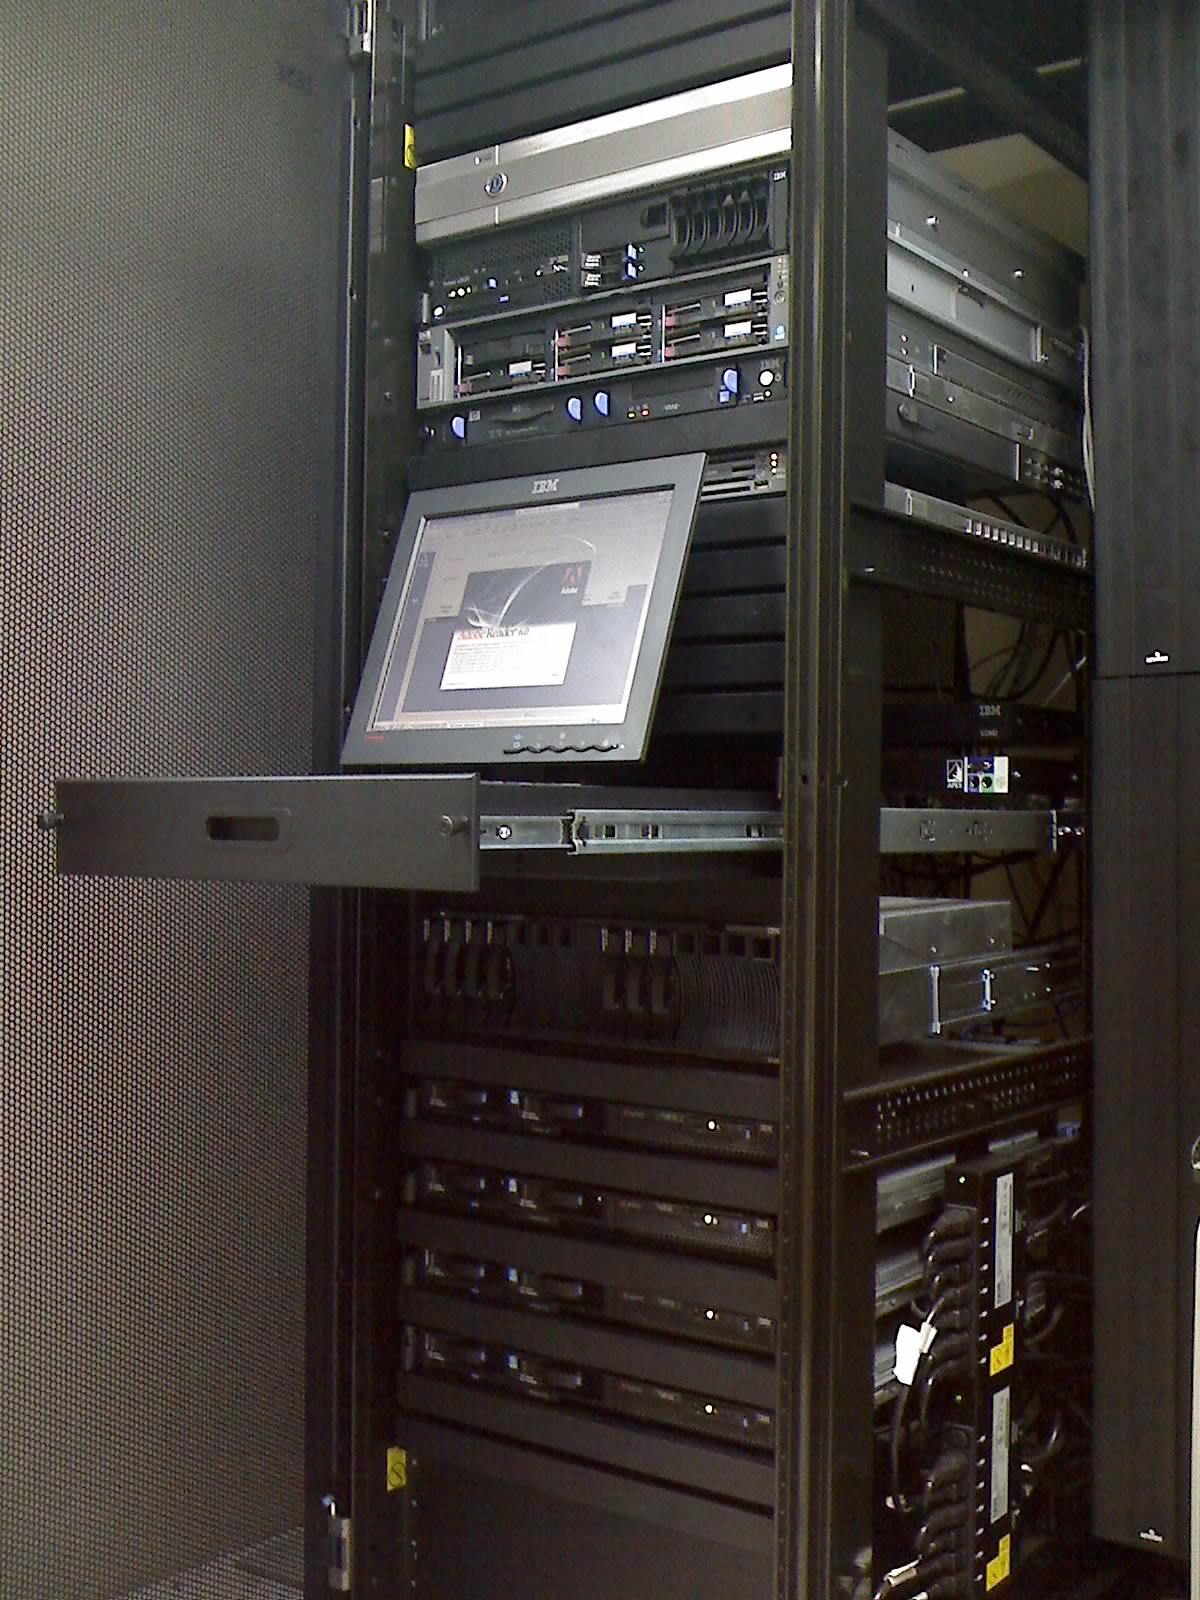
\includegraphics[width=0.75\linewidth]{Wiki_Rack001.jpg}
	\caption{Foto van Jfreyre afkomstig van \url{https://commons.wikimedia.org/wiki/File:Rack001.jpg}}
\centering
\end{figure}

Om hogere dichtheden te bereiken wordt er gebruik gemaakt van blade servers\index{Blade servers}. Bij blade servers zitten er meedere servers (blades) in \'e\'en fysieke behuizing (19''-kast). De servers delen een backplane, de voeding(en) en de behuizing waardoor er effectief meer servers passen op dezelfde oppervlakte. Een nadeel van blades is dat de warmte ontwikkeling ook veel meer geconcentreerd wordt en dat kan leiden tot zogenaamde hotspots, wat slecht is voor de koeling.

\subsection{Server virtualisatie opdrachten}
\begin{enumerate}
\item Zoek op Internet naar een load balancer en schrijf een stuk over welke technieken er gebruikt worden op load balancers. Zijn er ook software oplossingen die je kan inzetten als load balancer?
\item Welke software is er beschikbaar om rekenclusters mee op te zetten?
\item Welke software moet je installeren om een Windows Cluster op te zetten?
\end{enumerate}

\section{Desktop Virtualisatie}\index{Desktop virtualisatie}
Wat we met servers kunnen, kunnen we natuurlijk ook met desktops. We kunnen een virtuele machine aanmaken en daarop een desktop OS installeren en dan met een applicatie deze desktop overnemen. Hierdoor worden over het netwerk alleen de toetsenbord en muis gegevens opgestuurd naar de virtuele machine en terug komt de beeldschem-informatie. De client kan dus met veel minder hardware toe.

Voor de beheerder zit de winst erin dat updates alleen nog op de server hoeven te worden uitgevoerd, waarbij hij het zelfs met \'e\'en image af zou kunnen, en dat bij een probleem de gebruiker naar een andere VM gestuurd kan worden terwijl de beheerder de problematische VM opknapt. Ook wordt er op deze manier weer effici\"enter met resources omgegaan. Er hoeft niet meer in elke machine een zware processor en geheugen te zitten, niet gebruikte resources kunnen verdeeld worden over de beschikbare VMs.

Een ander voordeel is dat de desktop op deze manier ook remote aangeboden kan worden aan gebruikers wat tele-werken of thuiswerken makkelijker maakt.

\subsection{VDI - Vitrual Desktop Infrastructure}\index{VDI}\index{Virtual Desktop Infrastructure}
VDI staat voor Virtual Desktop Infrastructure en is een uitvinding van VMware dat het in 2006 op de markt bracht. VMWare gebruikte zijn eigen technologie, VMWare ESXi, om daarop Windows XP virtual machines te laten draaien. Via de standaard Remote Desktop software van Microsoft waren deze desktops beschikbaar voor gebruikers. Het is een techniek om desktop systemen beschikbaar te stellen, waarbij de desktop computers vervangen kunnen worden door thin clients.

De clients verbinden aan de VM via een remote desktop protocol zoals Microsofts Remote Desktop Protocol (RDP) of Citrix ICA (Independent Computing Architecture) protocol. De protocollen sturen scherm afbeeldingen naar de client en de muis en toetsenbord gegevens naar de VM.

De Virtual Desktop Environment (VDE) draait volledig op de server en ook alle data blijft op de server. Een voordeel van VDI is dan ook dat als een eindgebruikersdevice wordt gestolen, dat alle gegevens op de server staan. Er kan dus bij diefstal geen of minder snel gevoelige informatie op straat komen te liggen. Een ander voordeel is dat omdat de VDE op de server draait de toegang tot deze omgeving niet gelimiteerd hoeft te zijn tot het bedrijfspand, maar de desktop omgevingen ook beschikbaar gesteld kunnen worden aan thuisgebruikers via bijvoorbeeld een VPN (Virtual Private Network) verbinding.

VDI bestaat er in 2 smaken, persistent VDI en non-persistent VDI. Bij persistent VDI gedraagt de desktop zich zoals we ook van een installatie op een eigen machine verwachten. De wijzgigingen aan de achtergrond, de kleuren en andere zaken worden opgeslagen op het systeem. Elke keer als de gebruiker inlogd op een persisten VDI desktop ziet zijn omgeving eruit zoals deze het heeft achtergelaten.

Een non-persistent VDI zorgt ervoor dat bij elke nieuwe connectie de desktop eruit zoals dat ingesteld is door de beheerder. Wijzigingen door gebruikers worden dus niet opgeslagen. Deze laatste oplossing is goedkoper en eenvoudiger dan de non-persistent VDI oplossing.


\subsection{RDS - Remote Desktop Service}\index{RDS}\index{Remote Desktop Service}
Het RDP (Remote Desktop Protocol) luisterd standaard op port 3389. Het protocol is ontwikkeld door Microsoft op basis van het ITU T.128 protocol. De versie van Microsoft is gepatenteerd door Microsoft. Het protocol geeft de mogelijkheid tot het overnemen van systemen en het meekijken bij en het ondersteunen van gebruikers.

RDP geeft de gebruiker de mogelijkheid om ook geluid naar de desktop te sturen. Lokale bestanden, printers en interfaces kunnen gebruikt wordt op de remote desktop. Ook knippen en plakken tussen de lokale en de remote omgeving is mogelijk.


\subsection{ICA - Independent Computing Architecture}\index{ICA}\index{Independent Computing Architecture}
De Independent Computing Architecture ofwel ICA is een proprietary protocol van Citrix Systems. Het independent betekent dan ook niet dat het een open standaard is, maar voor het feit dat het beschikbaar is op verschillende computer systemen en dus niet gebonden is aan een specifiek platform (lees Windows).

ICA gebruikt standaard port 1494.

\subsection{Nadelen desktop virtualisatie}
Het aanbieden van gevirtualiseerde desktops kent zijn nadelen. Voor elke gelijktijdige gebruiker in een organisatie moet er een virtual machine aanwezig zijn. Dit kan oplopen tot honderden of duizenden virtuele machines die via het netwerk ontsloten moeten worden. Dit vraagt veel van de virtualisatie omgeving, maar ook van het netwerk en de opslagsystemen. Naast de gebruikersdata moeten ook alle virtual machine images opgeslagen worden. Het loont dus om deze images zoveel mogelijk uit te kleden, tot het absolute minimum.

De initi\"ele kosten zijn hoog. Er zijn zware servers nodig om de desktops virtueel te kunnen draaien, er zijn extra licenties nodig voor de software en er blijven nog steeds eindgebruikers devices nodig, zoals thin clients of laptops, om de virtuele desktops te kunnen benaderen.

Een ander probleem dat vaak ontstaat is het gebruik van de lokale functionaleiten van het access device. Denk dan bijvoorbeeld aan het gebruik van USB-sticks of het kunnen draaien van muziek. De USB-stick moet gekoppeld kunnen worden aan de remote desktop en het geluid van de remote desktop player moet hoorbaar zijn op het access device.

Een laatste nadeel is het anytime, anyplace, anywhere, probleem. Zonder degelijke Internet verbinding is het gebruik van een remote desktop niet mogelijk, of zo traag dat we er niet op willen werken.

Een probleem dat specifiek is voor desktop virtualisatie is de vraag om goede resoluties door de gebruikers. Hoe hoger de resoluties hoe beter de grafische kaart moet zijn die in de hypervisor zit. Voor de beste resoluties moet de hypervisor voorzien zijn van een GPU die dan geshared aangeboden kan worden aan de VMs. Het is ook mogelijk om een GPU dedicated aan te bieden aan een VM, maar dan wordt het wel een dure oplossing, want dan moet er voor elke VM een GPU kaart aanwezig zijn. Een andere oplossing is het emuleren van een GPU. Dit is performance technisch niet de beste oplossing, maar wel de goedkoopste.


\subsection{Remote Desktop Opdracht}
\begin{enumerate}
\item Zet een virtual machine op en installeer Windows 10. Enable RDP en connect vanaf je laptop via de RDC naar je VM.
\end{enumerate}

\section{The Cloud: Virtual Private Servers}\index{VPS}\index{Virtual Private Server}

\chapter{Webhosting (PaaS)}\index{PaaS}\index{Webhosting}
\section{LAMP}\index{LAMP}

\chapter{Applicatie Virtualistie (SaaS)}\index{SaaS}\index{Applicatie virtualisatie}
Steeds meer diensten draaien in de cloud, om deze diensten aan te bieden draaien er op servers web-servers, database-servers en waarschijnlijk nog allerlei andere services die zorgen dat de totale infrastructuur draaien blijft.

\section{Citrix, Microsoft en VMWare}
\subsection{Citrix}
In 1995 bracht Citrix Systems een product met de name WinFrame op de markt. WinFrame was Windows NT 3.51 als multi-user systeem. Meerdere gebruikers konden tegelijkertijd ingelogd zijn op het systeem en daar applicaties opstarten. De applicaties "draaiden" over het netwerk. De applicaties zijn dus niet lokaal ge\"installeerd, maar alleen ge\"installeerd op de server. Op de client is alleen de ICA client software ge\"installeerd, dit kan op een Windows systeem zijn, maar ook bijvoorbeeld een Mac OS X systeem of Linux. Op deze manier kunnen Windows applicaties gedeeld worden.

Om WinFrame te ontwikkelen heeft Citrix een licentie genomen op de Windows broncode voor NT 3.51 en heeft aan deze broncode de aanpassingen gedaan om van Windows NT een multi-user OS te maken. De verbinding tussen WinFrame en de desktop client wordt gemaakt via het ICA protocol. WinFrame heeft in de loop van de tijd wat naamsveranderingen ondergaan. Het heeft onderandere MetaFrame, Presentation Server en XenApp geheten. Het is tegenwoordig op de markt als Citrix Virtual Apps.

De client applicatie heette vroeger Citrix Receiver en heet nu Citrix Workspace App, voor Linux wordt er vaak gesproken over de ICAClient.

Microsoft heeft de code van Citrix WinFrame gelicenseerd van Citrix en heeft daarmee Microsoft Terminal Server op de markt gebracht in Windows NT 4.0. Vanaf Windows 2008 R2 (2009) heet het product Remote Desktop Services.

\section{Hosted applications}\index{Hosted applications}
\section{Containerisatie}\index{Containers}
\section{Containerisatie software}\index{Containerisatie}
\subsection{LXC}\index{LXC}
\subsection{Docker}\index{Docker}
\subsection{Kubernetes}\index{Kubernetes}
\section{Cloud Applicaties}
\subsection{Google Apps}
\subsection{Microsoft Office 365}

%%%%%%%%%%%%%%%%%%%%%
%%% Index and End %%%
%%%%%%%%%%%%%%%%%%%%%
%\backmatter
\printindex
\end{document}

%%% Last line %%%
